\chapter{Neue Auswahlkomponenten}

% todo paragraph
{\color{red} \textbf{FEHLENDER PARAGRAPH KOMMT NOCH}}


\section{Design}

Das Design der neuen Auswahlkomponente ist stark vom Kolibri-Designsystem inspiriert, jedoch mit einigen Anpassungen, um die Lesbarkeit und Benutzerfreundlichkeit zu optimieren. 
Der Fokus liegt darauf, eine konsistente und ansprechende Benutzererfahrung zu schaffen, die sich über alle modernen Browser hinweg hält.


\subsection{Designansatz}

Die Gestaltung der Dropdown-Komponente basiert auf dem Designsystem Kolibri, um eine konsistente Benutzererfahrung zu gewährleisten. 
Kolibri bietet bereits ein umfassendes Set von Richtlinien und Komponenten, die es ermöglichen, Anwendungen einheitlich und benutzerfreundlich zu gestalten.


\subsection{Mögliche Designoptionen eines Elements}

{\color{red} \textbf{FEHLENDER PARAGRAPH KOMMT NOCH}}

% border, background-color, font-color, underline, italic, font-weight, line left side
% pro cons pro möglichkeit mit passenden farboptionen
% kombination 2er status eines elements

\clearpage
\subsection{Figma-Prototypen}

Zur Visualisierung und interaktiven Testing des Designs kam Figma zum Einsatz. 
Figma ist ein webbasiertes Tool zur Erstellung von UI/UX-Designs, das Echtzeit-Kollaboration ermöglicht. 
Durch die Nutzung von Figma konnten schnell Prototypen erstellt und diese mit Stakeholdern und Nutzern geteilt werden, um Feedback zu sammeln und Iterationen vorzunehmen.

Die folgenden Screenshots \ref{img:figmaPrototype1} bis \ref{img:figmaPrototype3} zeigen die in Figma erstellten Prototypen der Dropdown-Komponente:

\begin{figure}[!htb]
    \centering
    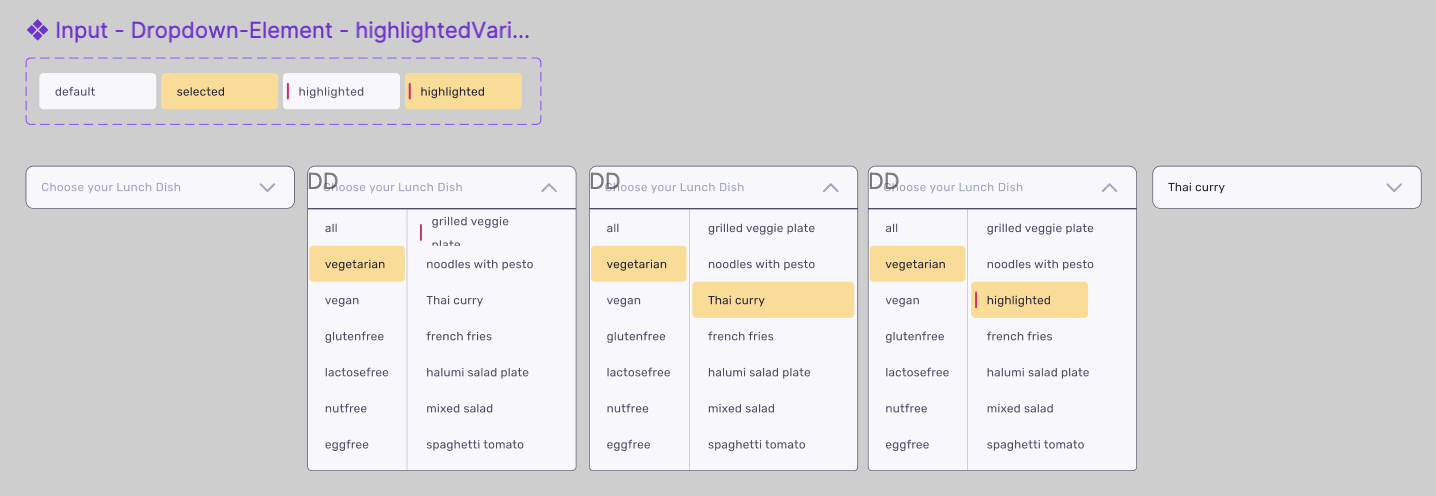
\includegraphics[width=100mm]{figma-prototype-1.png}
    \caption{Figma Prototyp - Dropdown Komponente 1}
    \label{img:figmaPrototype1}
\end{figure}

\begin{figure}[!htb]
    \centering
    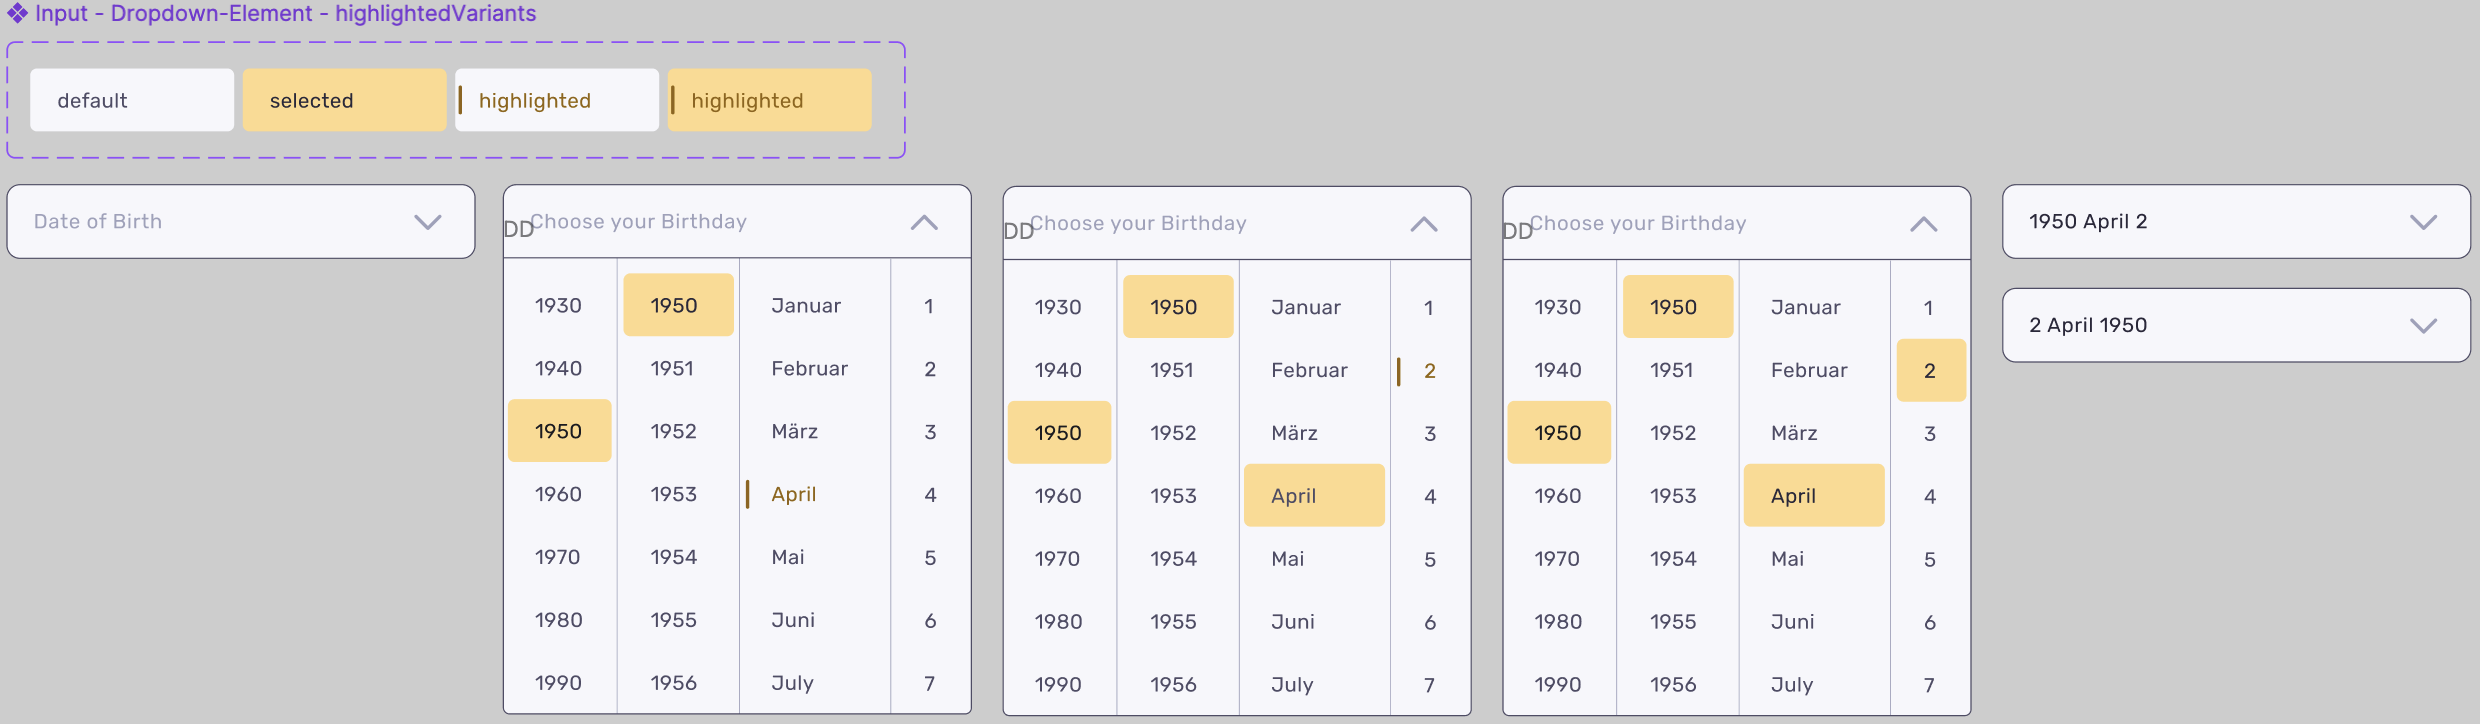
\includegraphics[width=100mm]{figma-prototype-2.png}
    \caption{Figma Prototyp - Dropdown Komponente 2}
    \label{img:figmaPrototype2}
\end{figure}

\begin{figure}[!htb]
    \centering
    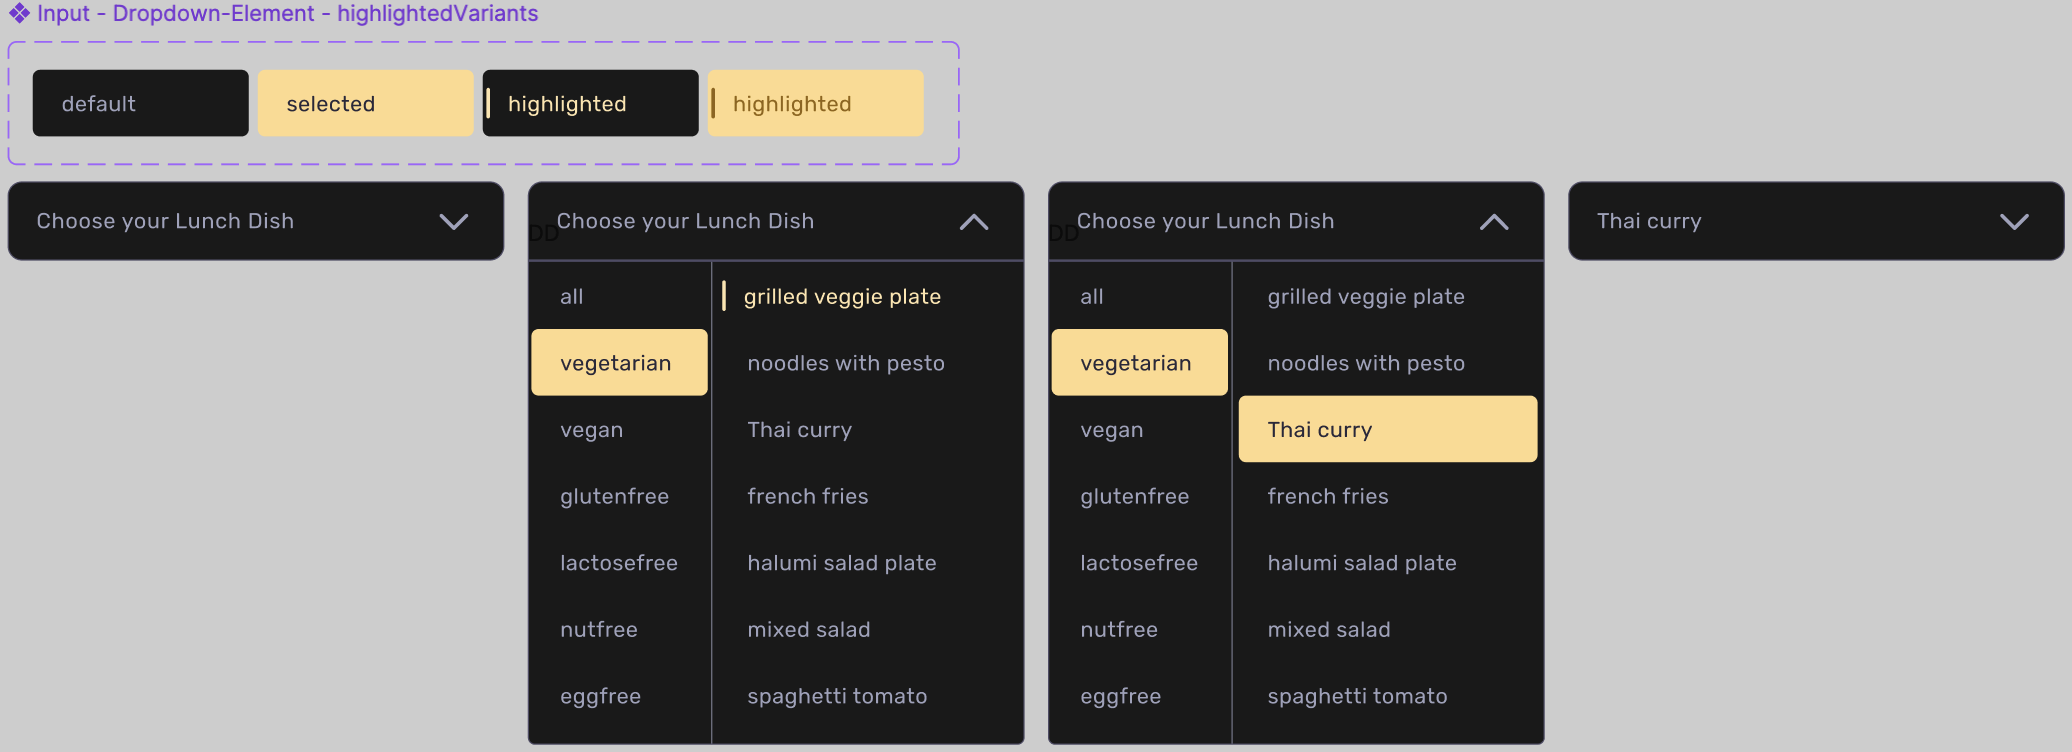
\includegraphics[width=100mm]{figma-prototype-3.png}
    \caption{Figma Prototyp - Dropdown Komponente 3}
    \label{img:figmaPrototype3}
\end{figure}


\subsection{Farbpalette und Kontrast}

Während das Kolibri-Designsystem eine Vielzahl von Farben bietet, wurden spezifische Anpassungen vorgenommen, um sicherzustellen, dass die Dropdown-Komponente gut lesbar ist. 
Um eine bessere Nutzerfreundlichkeit zu erhalten, gestaltet sich die Farbauswal (Abbildung \ref{img:designColors}) so, dass sie hohen Kontrast bietet und somit die Barrierefreiheit der Anwendung verbessert.

\begin{figure}[!htb]
    \centering
    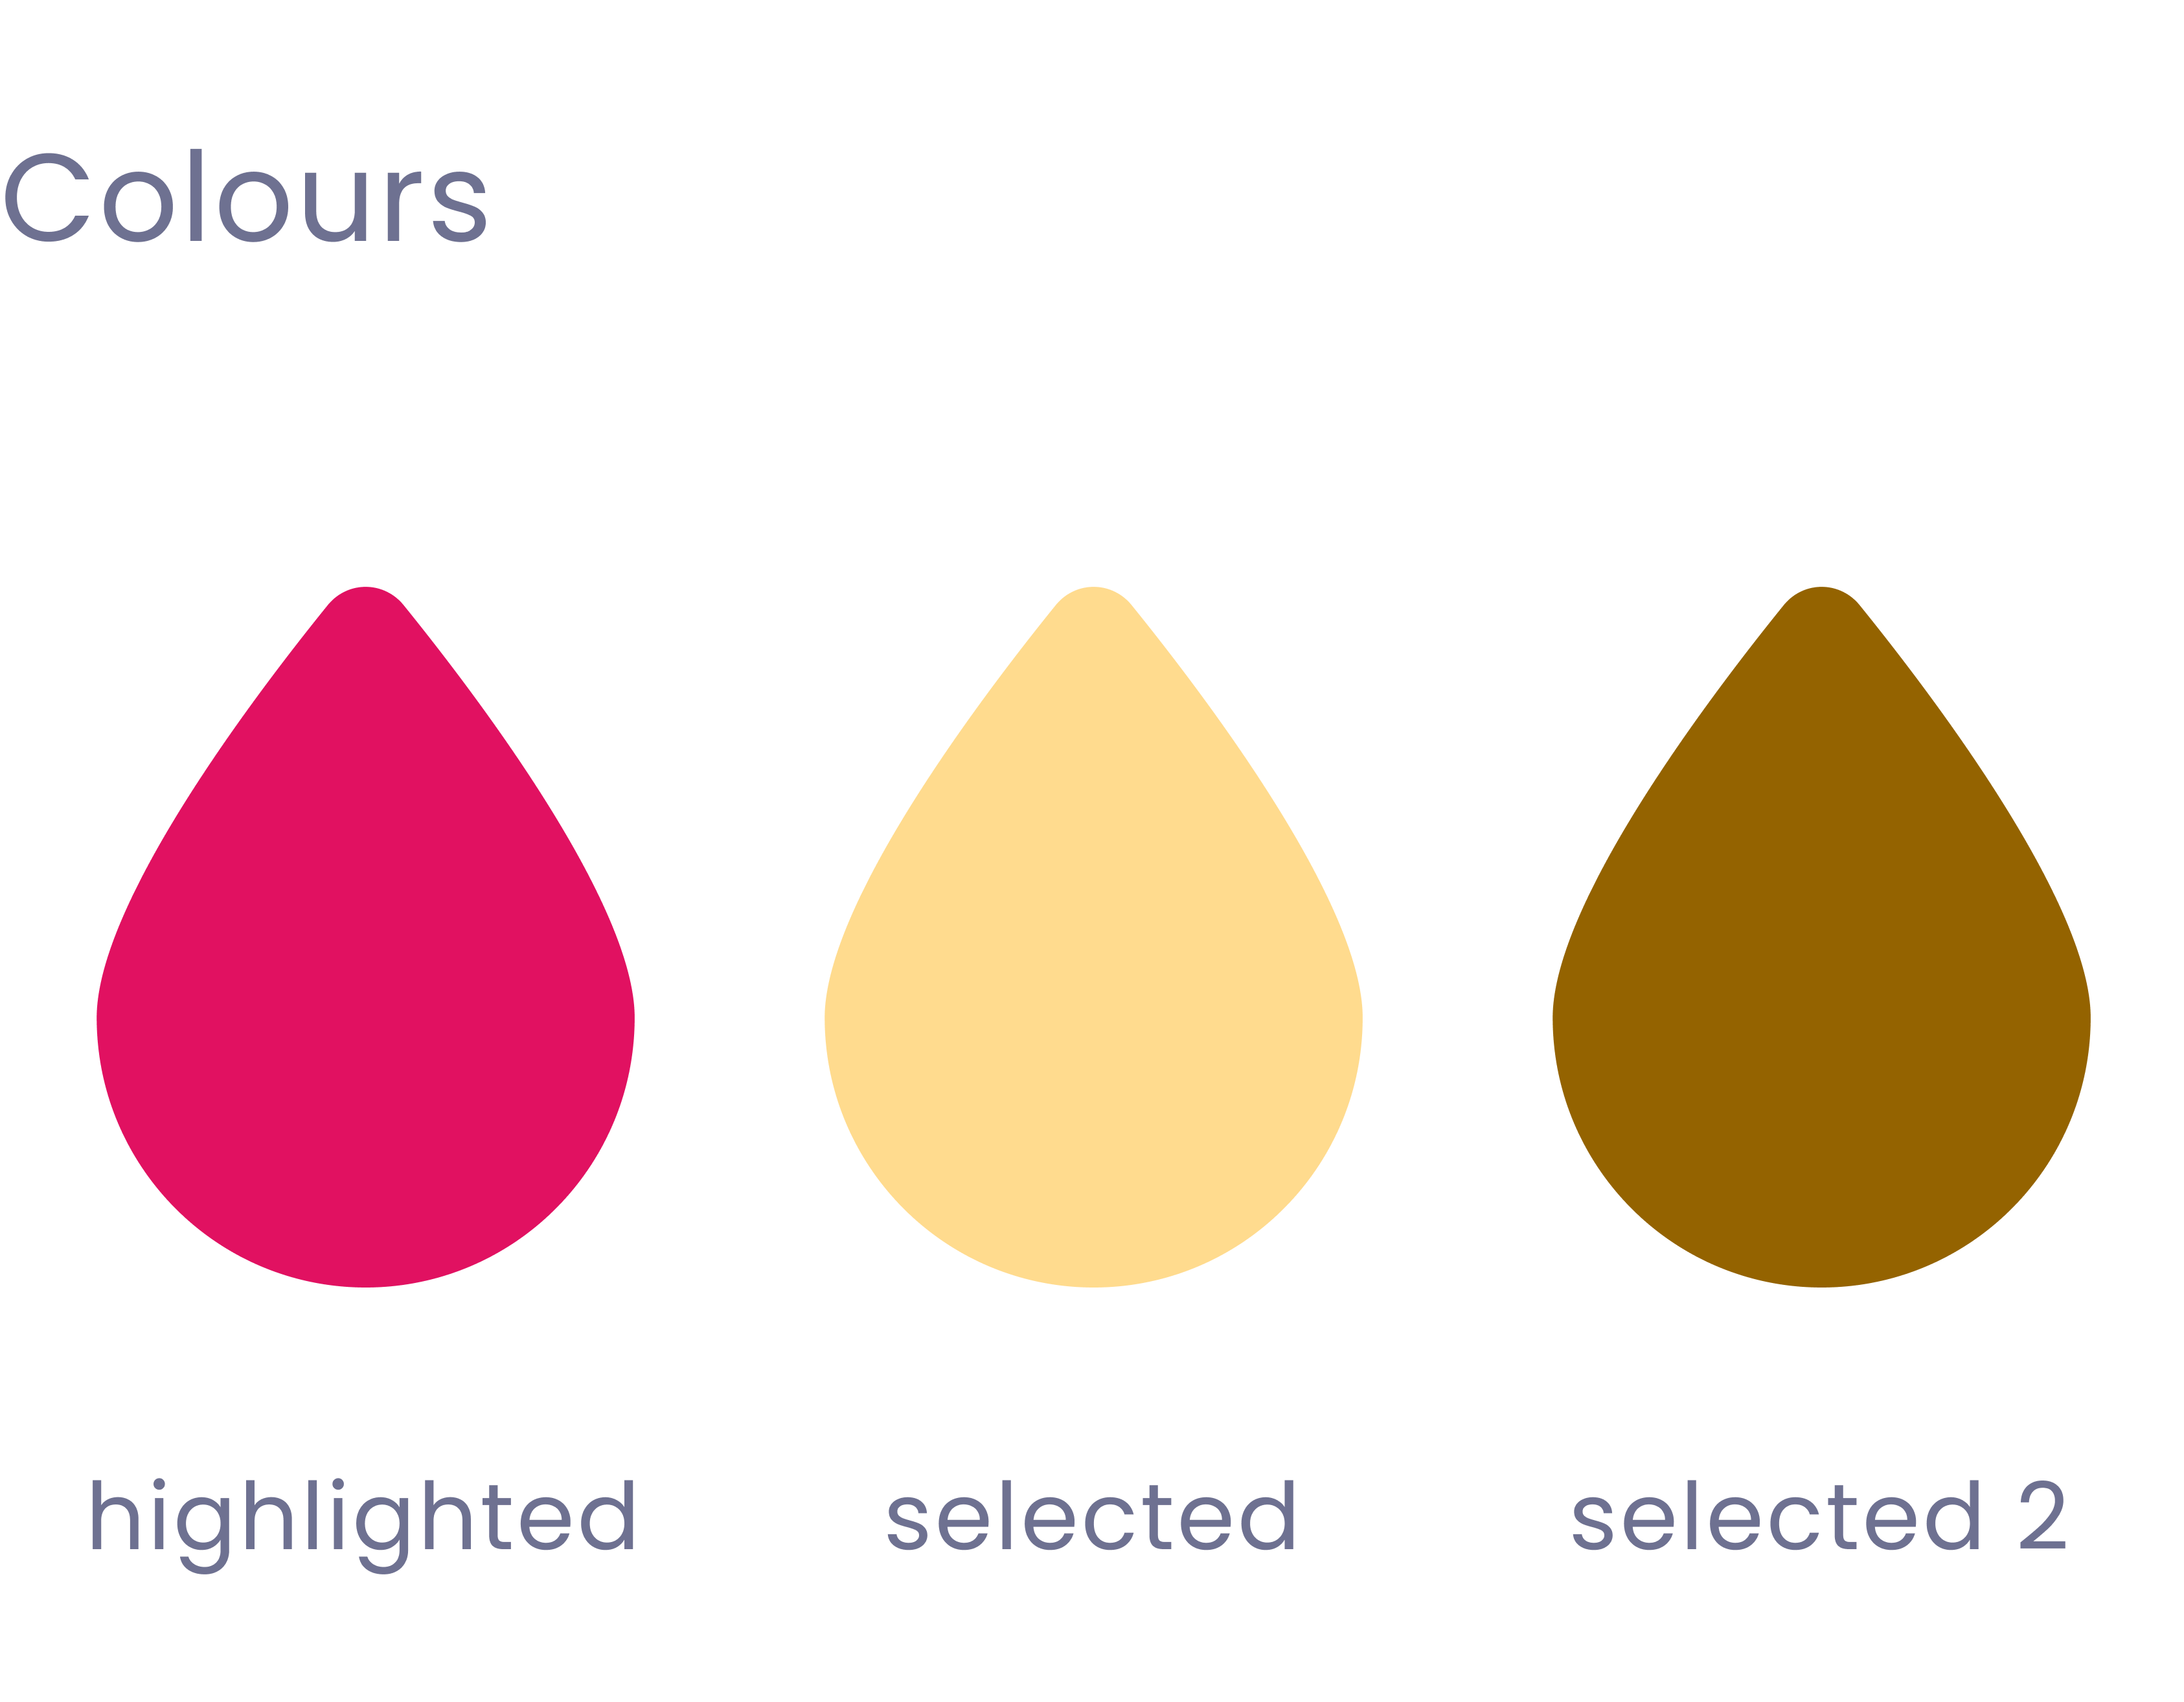
\includegraphics[width=70mm]{design-colors.png}
    \caption{Kolibri Design System - Farbpalette}
    \label{img:designColors}
\end{figure}

\noindent
Die originalen Farben erhalten im neuen Dropdown eine angepasst Verwendung:

\begin{itemize}
    \item \textbf{Original} $\rightarrow$ \textbf{Neu}
    \item Kolibri-Light/Yellow/300 $\rightarrow$ selected
    \item Kolibri-Light/Danger/--kb-danger-accent $\rightarrow$ highlighted
    \item Kolibri-Light/Warning/--kb-warning-dark $\rightarrow$ cursor position
\end{itemize}

\noindent
Der Code \ref{code:cssImports} zeigt die importierten CSS-Dateien, die als Grundlage für dieses Styling dienen:

\begin{lstlisting}[style = htmlcssjs, caption = CSS Imports, label = code:cssImports]
@import "../../../css/kolibri-base.css";
@import "../../../css/kolibri-light-colors.css";
\end{lstlisting}


\subsection{Layout und Typografie}

Um die in Figma entworfenen Designs umzusetzen, erhält die Dropdown-Komponente eigenes CSS.
Nachfolgend im Codeausschnitt \ref{code:styleDemoPage} ist der relevante CSS-Code, der zur Gestaltung der Dropdown-Komponente verwendet wird:
% todo code passt nicht zu text => code ist in selectprojector / columnoptionsprojetor jeweils unten
% todo reduzieren auf wesentliche stellen & beschreiben

\begin{lstlisting}[style = htmlcssjs, caption = style.css der Demo-Page, label = code:styleDemoPage]
body {
    perspective: 100vw;
}

.card {
    max-width:  40em;
    margin:     1em auto 2em auto;
    padding:    2em 4em;
    box-shadow: var(--kolibri-box-shadow);
    min-width:  620px;
}

h1 {
    text-align:  center;
    font-family: var(--font-sans-serif), sans-serif;
    margin-top:  0;
}

h3, h4 {
    margin-top: 3rem;
}

.holder {
    min-width: 160px;
    width: fit-content;
    margin: 1rem 0;
}

.holder > div {
    margin: 0;
    width: 100%;
}
\end{lstlisting}


\subsection{Interaktionsdesign}

Die Dropdown-Komponente ist so gestaltet, dass sie sowohl für Maus- als auch Tastaturbenutzer optimal funktioniert. 
Das Design der Interaktionen bietet eine intuitive und leicht zugängliche Bedienung der Komponente.
Um die Benutzerführung zu erleichtern, erhalten die hervorgehobenen (highlighted) bzw. ausgewählten (selected) Optionen eine Kennzeichnung durch spezifische CSS-Klassen.
Der CSS-Code \ref{code:styleExample} zeigt einen Style-Ausschnitt auf ein gehighlightetes Element.

% todo insert correct code in highlight
\begin{lstlisting}[style = htmlcssjs, caption = Style Beispiel für Zustand Highlight, label = code:styleExample]
.highlighted {
    background-color: #e0e0e0; 
}
\end{lstlisting}


\subsection{Komponentengrösse und Layoutanpassungen}

Mit der Definition von Mindest- und Maximalbreite sowie flexiblen Layouts ist sichergestellt, 
dass die Dropdown-Komponente auf verschiedenen Bildschirmgrössen funktioniert und sich gut darstellen lässt.

% todo code wieder für demo und nicht komponte => ändern & beschreiben
\begin{lstlisting}[style = htmlcssjs, caption = Flexible Layouts für Demo-Page, label = code:layoutDemoPage]
#componentCity .select-input-component {
    min-width:  400px;
}

#componentImg .select-input-component,
#componentCountry .select-input-component {
    min-width:  320px;
}

#componentImg .options-column {
    width: auto;
}

#componentImg img {
    width:  2rem;
    max-height: 1.3rem;
    object-fit: contain;
}

form {
    display: flex;
    gap: 2rem;

    > button {
        border-radius: 5px;
        color: white;
        background-color: var(--kolibri-color-output);
        font-weight: bold;
        outline: none;
        border: none;
        padding: .5rem;

        &:focus {
            filter: brightness(150%);
        }
    }
}

label {
    display: flex;
    align-items: center;
}
\end{lstlisting}


\subsection{Benutzerfeedback und Prototyping}

Der Einsatz von interaktiven Figma-Prototypen ist hilfreich beim Evaluieren der initialen Benutzerfreundlichkeit und intuitiven Bedienung. 
Mit der Integration der Rückmeldungen von Benutzerinteraktionen in das Design verbessert sich die Usability kontinuierlich.
Beispiele für die Prototypen und verschiedene Zustände der Dropdown-Komponente ist im oberen Hälfte des Bildes \ref{img:figmaPrototype1} ersichtlich.

Die Gestaltung der Auswahlkomponente umfasst sowohl visuelle als auch funktionale Aspekte. 
Gezielte CSS-Anpassungen und ein durchdachtes Interaktionsdesign finden in der Realisierung ihren Platz. 
Das Ziel ist, eine ansprechende und benutzerfreundliche Komponente zu schaffen. 
Sie fügt sich nahtlos in das Kolibri-Designsystem ein und überzeugt gleichzeitig durch optimierte Les- und Bedienbarkeit.


\section{Interaktionen}

Damit ein gemeinsames Verständis entsteht, gilt es für die Bedienung der Komponente Regeln festzulegen.
Wie in den Grundlagen bereits beschrieben kann sich ein Wert aus dem Optionen-Container in verschiedenen Zuständen befinden.
In diesem Absatz spielen Selektion, Highlight und Cursor Position eine Rolle.
Zur Auffrischung: 

\begin{itemize}
    \item \textbf{Selektion}: Ausgewählter Wert der Spalte
    \item \textbf{Highlight}: Element unterhalb des Mauszeigers
    \item \textbf{Cursor Position}: Position (Element) der Tastatur
\end{itemize}

\noindent
Bei der Festlegung der Maus-Interaktion fiel die Entscheidung auf folgendes:

\begin{itemize}
    \item \textbf{mouseover}: visuelles Highlighting des Elements ohne Selektionsänderung
    \item \textbf{click}: Änderung der Cursor Position \& direkte Selektionsänderung
\end{itemize}

\noindent
Die Tastatur-Steuerung mit den Pfeiltasten hingegen hält sich an diese Bedienungen:

\begin{itemize}
    \item Änderung der Cursor Position
    \item \textbf{selbe Spalte}: direkte Selektionsänderung ohne weitere Bestätigung
    \item \textbf{Spaltenänderung}: keine Selektionsänderung
\end{itemize}

\noindent
Anhand dieser Regeln entstanden folgende Aktionen als Basis für den ersten Projektor der neuen Komponente. 


\clearpage
\import{../tables}{d.newComponent.tex}

Das Undo und das Redo auf der Komponente erhält im ersten Projektor keine spezielle Definition.
Gewisse Verhaltensweisen finden sich im geschlossenen als auch offenen Zustand der Komponente wieder.
Anders als bei den existierenden Komponenten, ist bei der Neuen die Leertaste neu belegt. 
Ist die Liste bereits offen, wird der sich aktuell unter der Cursor Position befindliche Wert selektiert.
Die Interaktionen können in weiteren Projektoren angepasst bzw. geändert werden.


\section{Prinzipien \& Regeln}

Um stabilen und verständlichen Code zu garantieren, hält sich dieses Projekt an diverse Prinzipien.
Ein Ansatz ist alle Objekte so immutable als möglich zu halten.
Dadurch können unerwartete Änderungen vermieden werden.
Weiter gilt es, die Bestandteile im KISS-Stil umzusetzen.
Dazu zählt, dass die einzelnen Objekte und Funktionen möglichst privat zu gestalten sind.
Die Bausteine sind kurz und übersichtlich aufzubauen.
Zu diesem Zweck soll Separation of Concern eingesetzt werden, so dass jede Funktion nur eine Aufgabe zu erfüllen hat.
Damit der Code einfach und lesbar bleibt bzw. wird, gilt es, Entscheidungen zu treffen.
Zu diesen Entschlüssen zählt das bewusste Weglassen von Funktionalität und somit auch Komplexität.

Beim implementieren ist darauf zu achten, den Code sauber zu formatieren.
Zudem ist es sinnvoll, die Änderungen regelmässig mit dem Code-Analyse-Tool von Intellij auf ihre Qualität zu prüfen. 
Diese Prinzipien und Regeln unterstützen eine ordentliche Entwicklungsumgebung für eine stabile Komponente.
Das Kapitel Patterns bietet eine weitere Möglichkeit den Code strukturiert zu halten.


\section{Patterns}

In diesem Projekt finden sich einige Code-Patterns wieder.
Die Wichtigesten wie Null-Object, Projector und Decorator sind in den nachfolgenden Unterkapitel genauer erläutert.
Eine weitere Rolle spielt unter anderem die Master-Detail-View, aber im Zusammenhang mit der Komponente eher nebensächlich.
Zudem ist die Anwendung nicht typisch bzw. genau abgegrenzt.
Die Implementation erhält durch die verwendeten Patterns eine Struktur und läuft stabiler.


\subsection{Null Object Pattern}

Ein Pattern, welches im Verlauf der Arbeit eine wichtige Rolle eingenommen hat, ist das Null-Object Pattern.
(\cite{nullObjectPattern}) Null hat den Nachteil, dass alle Funktionsaufrufe darauf zu Fehlern führen.
Das Null-Object besteht aus vordefinierten Default-Werten und besitzt Do-Nothing-Implementationen für alle Funktionen.
Durch die Verwendung dieses speziellen Objekts entfällt eine ansonsten notwendige Nullwertprüfung.
Zudem ist jedes erstellte Null-Object wertegleich.

Um eine Selektion zurücksetzen zu können, muss diese Komponente eine Null-Option enthalten.
Die Verwendung des Null-Objects findet sich an mehreren Stellen des Codes wieder.
Die Definition der angewendeten Null-Option zeigt der nachfolgende Code.

\begin{lstlisting}[style = htmlcssjs, caption = Null-Option, label = code:nullOption]
/** @private @returns { OptionType } */
const reset = () => {
    return Option(null, null);
};

/** @public @type { OptionType } */
const nullOption = reset();
\end{lstlisting}

Hierbei muss nur die $nullOption$ selbst exportiert werden und das Reset bleibt $private$.
Um die selbe Funktionalität wie die gewünschten Objekte zu bieten, erhält diese Konstante den Typ $Option$.
Der Codeausschnitt \ref{code:nullOption} befindet sich in der Datei $optionsModel.js$.
Mehr zur File Aufteilung ist in den nächsten zwei Unterkapiteln zu lesen.

\subsection{Projector Pattern}
% todo change ref to könig
(\cite{projectorPattern}) Das Projector Pattern basiert auf dem verbreiteten Model-View-Controll Pattern.
Das Model verwaltet die Daten, welche dargestellt werden sollen.
Zudem enthält die Komponente des Patterns die Geschäftslogik und verarbeitet die Regeln und Anfragen für die Daten.
Ein Controller generiert privat gehaltene Modelle.
Dabei werden nur die notwendigen Funktionen zur Verfügung gestellt.
Diese Funktionen können Getter, Setter und Listener der observierten Modelle und Werte sein.
Der Projektor bindet Daten-Modelle über den Controller an die View.
Auf der anderen Seite wird die View an die Models gebunden, dies erneut durch die Verwendung des Controllers.
Aus den Bindings und den Daten generiert ein Projetor die passende View.
Die View ist passiv und hat keine Kenntnis über die anderen Komponenten.

Dieses Pattern zeigte sich als eines der Wichtigsten für die Erstellung der neuen Komponente.
In den folgenden Grafiken sind Models als Zylinder, Controller als schiefes Rechteck und Projectors als Oval dargestellt.
Die Raute mit Option ist ein Daten-Typ, der über das gesamte Projekt seine Anwendung findet.
Das $starter.js$ beinhaltet alle Bestandteile, welche für eine Anwendung benötigt werden.
Das Puzzle wird im späteren Unterkapitel Decorator Pattern genauer beschrieben.
Die erste Implementation, welche dieses Pattern verwendet, ist auf Abbildung \ref{img:DiagramSelectComponentOld}.

\begin{figure}[!htb]
    \centering
    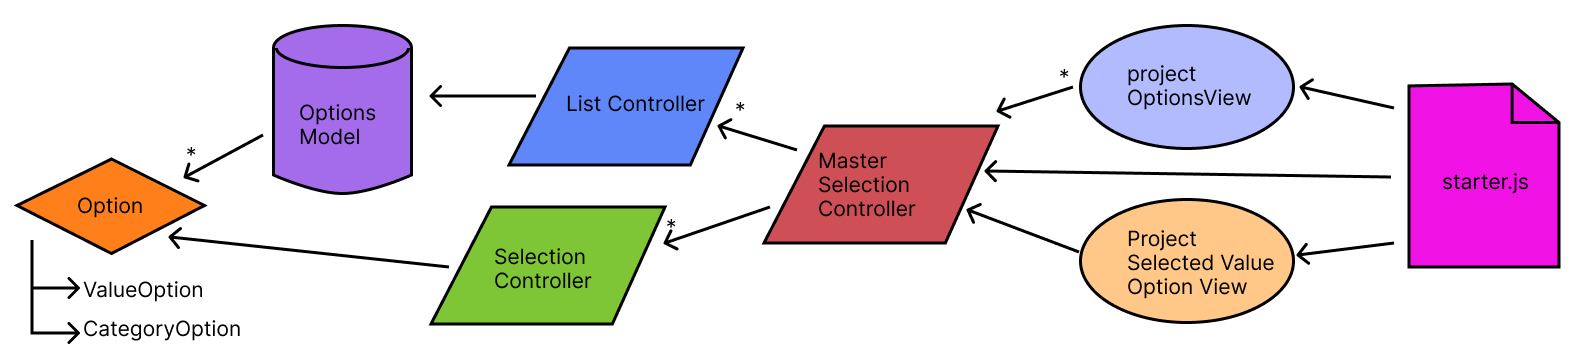
\includegraphics[width=120mm]{diagram-select-component-old.png}
    \caption{Diagramm Select Component - 1. Version}
    \label{img:DiagramSelectComponentOld}
\end{figure}

Diese Version zeigt noch viel Komplexität und duplizierenden Code in den einzelnen Funktionen.
Eine genaue Analyse der Komponente zeigt, dass sich das Pattern zwei Mal anwenden lässt.
Die neue Aufteilung ergibt die zwei folgenden Abbildungen \ref{img:DiagramColumnComponent} und \ref{img:DiagramSelectComponent}.
Die Implementation der dargestellten Diagramme resultiert aus einem Refactoring im grösseren Rahmen.

\begin{figure}[!htb]
    \centering
    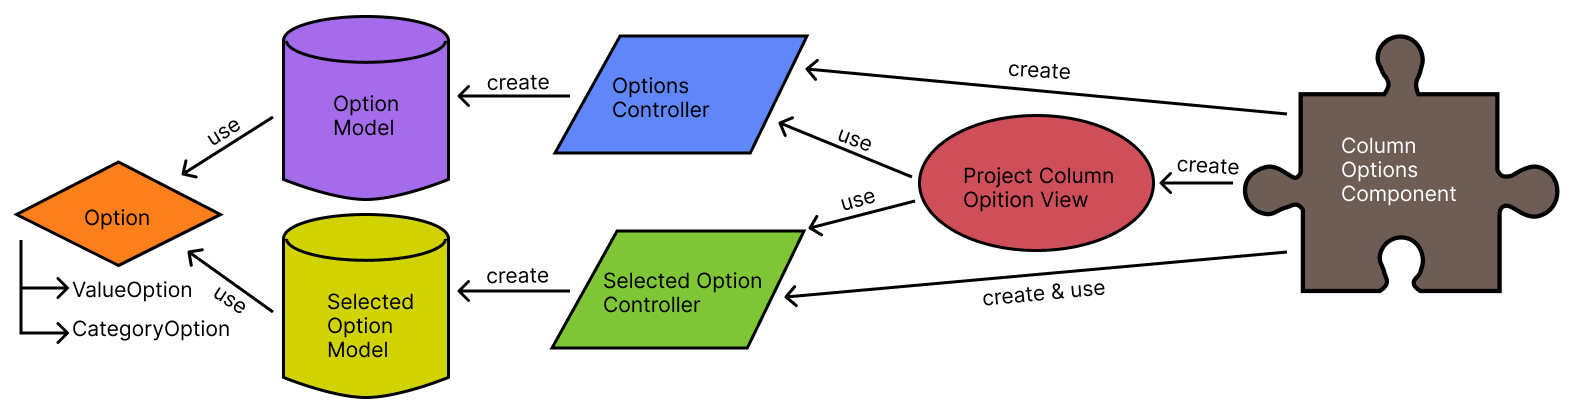
\includegraphics[width=120mm]{diagram-column-component-with-desc.png}
    \caption{Diagramm Column Component}
    \label{img:DiagramColumnComponent}
\end{figure}

Zum einen findet sich das Projector Pattern in einer einzelnen Spalte in der Options-Liste wieder.
Pro Kolonne existiert eine Auswahl und eine Menge von Optionen.
Diese beiden Bestandteile besitzen je ein eigenes Model und einen eigenen Controller.
In diesem Fall generiert der Projektor eine gemeinsame View mit Bindings zu den beiden Controllern.
Bei einer Anwendung übernimmt die $ColumnComponent$ die Verwaltung gewisser Bausteine (Mehr dazu später).

\begin{figure}[!htb]
    \centering
    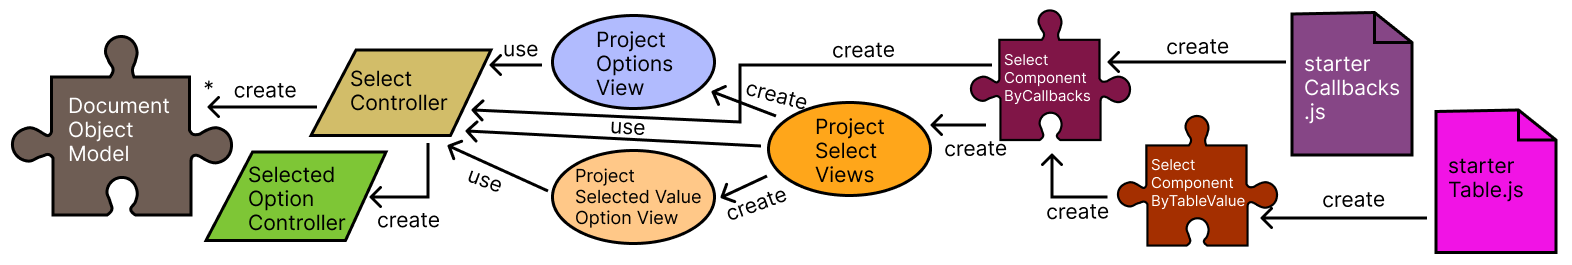
\includegraphics[width=120mm]{diagram-select-component-with-desc.png}
    \caption{Diagramm Select Component}
    \label{img:DiagramSelectComponent}
\end{figure}

Die Anwendungskomponente einer Column findet sich als Bestandteil des zweiten Projector Pattern wieder.
Ein $SelectController$ verwaltet eine bis mehrere $ColumnComponent$s als auch ein Element für die Tastaturnavigation.
Die sogenannte Cursor Position verwendet im Hintergrund ebenfalls einen $SelectedOptionController$. 
Dieser ist der selbe wie in der Abbildung \ref{img:DiagramColumnComponent} und findet hier eine Wiederverwendung.
Um die Bindings zu definieren, greifen die einzelnen Projektoren auf den selben Controller zu.
Der Master-Detail-Aufbau der neuen Komponente findet sich in der Aufteilung der Projektoren wieder.
Der Detail-Baustein kümmert sich um die aktuelle Auswahl und das Eingabefeld.
Die Master-Komponente verwaltet alle Spalten mit den Kategorie- und Werte-Optionen, sowie dessen Bindings.
In einer weiteren Funktion werden die beiden Projektoren zusammengeführt und in eine gemeinsame View eingebettet.
Auch diese Projector Pattern Anwendung schliesst mit einer Component - der SelectComponent - ab.
Mehr zu dieser und der Column-Component steht im nächsten Kapitel.


\subsection{Decorator Pattern}

(\cite{decoratorPattern}) Ein Decorator bietet zusätzliches Verhalten ohne das Originale Objekt zu verändern.
Zudem können verschiedene Funktionen kombiniert werden.
Dieses Pattern ermöglicht die Erstellung eines modularen und anpassbaren Codes.
In diesem Projekt unterstützt es die Gestaltung und Erweiterung der Auswahlkomponente.

Wie im vorherigen Kapitel erwähnt, besteht die neue Komponente unter anderem aus zwei sogenannten Component-Bausteinen.
Die Decorator sind in den Abbildungen \ref{img:DiagramColumnComponent} und \ref{img:DiagramSelectComponent} als Puzzle dargestellt.
Diese Bestandteile kombinieren die Funktionalität des Controllers mit der Erstellung der View.
Dadurch lässt sich die neue Komponente einfacher anwenden.

\begin{lstlisting}[style = htmlcssjs, caption = SelectComponentByTableValue dekoriert SelectComponentByCallback, label = code:componentDecorator]
const SelectComponentByTableValues = (
    selectAttributes,
    optionsTable,
    sortColumnOptionsAlphabetical = false
) => {
    /* code for mapping between table and callbacks */
    const component = SelectComponentByCallbacks(selectAttributes, callbacks);
    return {
        ...component,
    };
};
\end{lstlisting}

Ein weiterer Einsatzort ist bereits in der Abbildung \ref{img:DiagramSelectComponent} aus dem Vorkapitel zu erahnen.
Der rotbraune $SelectComponentByTableValue$ in Code \ref{code:componentDecorator} dekoriert die $SelectComponentByCallback$.
Damit bietet die neue Komponente zwei verschiedene Möglichkeiten der Anwendung.
Das nächste Kapitel geht genauer auf den Master-View-Bereich des $SelectProjector$s - Abbildung \ref{img:DiagramSelectComponent} - ein.


\section{Dropdown-Container}

Um alle Optionen zu gegebener Zeit darzustellen, stehen verschiedene Varianten zur Auswahl.
Eine Möglichkeit ist, den Container als HTML-Dialog zu gestalten.
Die vorhandenen Funktionen sind jedoch nicht für diese Komponente geeignet.
Für den gewünschten Zweck erfordert das Dialog-Element noch einiges an benutzerdefinierter Anpassung.

Eine weitere Variante ist, ein normales $div$ als Options-Container zu verwenden.
Dies erfordert ebenfalls einen enormen Implementationsaufwand.
Eine Andwendung dieses Ansatzes findet sich in der ersten Version der Komponente.
Hierbei eröffnet sich das Problem von der Inkonsistenz zwischen UI und Controller.
Zudem ist es möglich, dass unerwünscht mehrere Dropdown-Container gleichzeitig offen sind.

Als dritte Möglichkeit bietet sich die Popover-API an, welche seit 2024 von allen gängigen Browser unterstützt wird.
Durch das Refactoring der Variante mit dem normalen Div-Container resultiert eine Version mit der Anwendung dieser API.
Der Zusatzaufwand reduziert sich im Gegensatz zu den beiden oben erwähnten Container-Implementationen.
Der Grundaufbau des Popover-Container ist im folgenden Code \ref{code:PopoverExample} dargestellt.

\begin{lstlisting}[style = htmlcssjs, caption = Popover-Container Beispiel, label = code:PopoverExample]
<div popover="auto"
    id="select-component-0-options" 
    class="options-component" 
> </div>
\end{lstlisting}

Bei diesem Codeausschnitt ist wichtig, dass das Attribut $popover$ den Wert $auto$ erhält.
Dies bewirkt, dass die Popover sich automatisch schliessen, wenn ein Klick ausserhalb des Container passiert.
Das Öffnen und Schliessen des Dropdown-Elements kann über das $popovertarget$-Attribut mit der Popover-Id\footnotemark auf der Bedienkomponente gesteuert werden.
\footnotetext{$id$-Attribut des Div-Containers mit dem Attribut $popover$}
Als Alternative dazu besteht die Möglichkeit, das Popover über JavaScript zu steuern.
Hierbei besteht die Möglichkeit auf den Status und das Event des Togglens zuzugreifen.
Diese Funktionalitäten erlauben den Controller konsistent zum UI zu halten.


\section{Performance}

Um eine gute Performance zu bieten, ist es notwendig den Aufbau-Prozess einer Webseite zu kennen.
Dieser Ablauf ist im Kapitel \textbf{Grundalgen} unter \textbf{Ablauf Parsing \& Rendering} genau beschrieben.
Die folgende Abbildung \ref{img:RenderingProcessRecap} zeigt den Prozess im Überblick.

\begin{figure}[!htb]
    \centering
    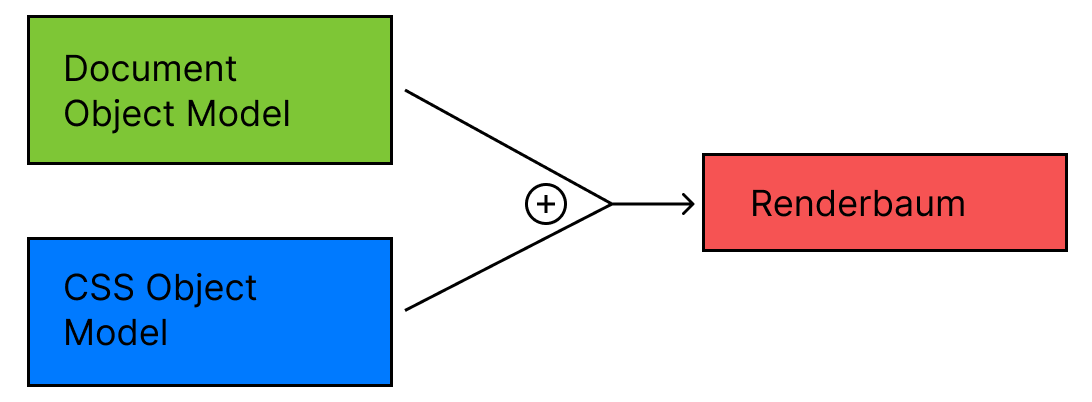
\includegraphics[width=120mm]{rendering-process.png}
    \caption{Rendering Prozess}
    \label{img:RenderingProcessRecap}
\end{figure}

Hierbei ist ein wichtiger Punkt, dass der Browser den Renderbaum (in der Abbildung \ref{img:RenderingProcessRecap} rot) maximal 60 Mal pro Sekunde neu zeichnen kann.
Daher müssen viele kleine Änderungen ausserhalb des Renderbaums - am besten in einem sogenannten Shadow-DOM - geschehen.
Ein Shadow-DOM ist ein Teilbaum, welcher nicht im Renderbaum angehängt ist.
Um dies zu bewerkstelligen, ist es sinnvoll, die Änderungen nach dem Abhängen des Elternknotens zu vollziehen. 
Nach den Änderungen kann der Teilbaum wieder an den gewünschten Ort platziert werden.

\begin{lstlisting}[style = htmlcssjs, caption = Performance Optimierung (columnOptionsComponent.js), label = code:PerformanceOptimization]
const addAllOptions = (options) => {
    const placeHolder = createHolder();
    columnView.replaceWith(placeHolder);
    if (options.length > 50) {
        setTimeout(() => {
            options.forEach((option) => {
                optionsController.addOption(option);
            });
            updateScrollbar(columnView);
            placeHolder.replaceWith(columnView);
        }, 80);
    } else {
        options.forEach((option) => {
            optionsController.addOption(option);
        });
        updateScrollbar(columnView);
        placeHolder.replaceWith(columnView);
    }
};
\end{lstlisting}

Code \ref{code:PerformanceOptimization} ist eine Stelle, die diese Technik verwendet.
Hier wird ein Platzhalter mit einem Lade-Indikator an die Ursprungsstelle gesetzt, damit der Nutzer ein Feedback erhält.
Sobald der SpaltenContainer abgekoppelt ist, lädt die Funktion die Optionen in den Shadow-DOM.
Nach Abschluss wird der Container mit den neuen Elementen an die originale Stelle zurückersetzt.

(\cite{efficientDomManipulation}) Weiter ist darauf achten, dass CSS-Klassen an Stelle von Inline-Styles verwendet werden sollten.
Das Cachen von mehrfach verwendeten Selektoren verbessert die Effizienz des DOMs.
Die Selektoren sollten hierarchisch möglichst flach und nicht verschachtelt sein.
Wenn es die Situation erlaubt, ist es besser, nicht mit $innerHTML$ zu arbeiten.
In diesem Projekt ist es für die Anzeige der Label jedoch nötig $innerHTML$ zu nutzen.
Dies liegt daran, dass ein Label auch ein Bild enthalten kann.
Generell verwendet die neue Auswahlkomponente keine Inline-Styles.
Die einzigen Ausnahme betrifft das verborgene Eingabefeld. 
Durch den Code \ref{code:InlineStyle} sind die Properties vor dem Überschreiben geschützt.

\begin{lstlisting}[style = htmlcssjs, caption = Inline-Style für Inputfeld, label = code:InlineStyle]
inputElement.setAttribute(
    "style", "all: unset !important; z-index: -1 !important; " +
    "position: absolute !important; inset: 5px !important; " +
    "color: transparent !important; pointer-events: none !important;"
);
\end{lstlisting}

Die Regeln in Code \ref{code:InlineStyle} sorgen dafür, dass das Input-Feld transparent als auch resetet ist.
Zudem befindet es sich im Hintergrund und besitzt dieselben Grösse wie der Container mit dem ausgewählten Wert.

\subsubsection{\color{dgray} Performance Vergleich}

Durch die Anpassungen der Performance Optimierung, verbesserte sich die Ladezeit bei grossen Datenmenge enorm.
Die Testseite enthält vier existierende und vier neue Auswahlkomponenten mit den selben Inhalten wie je eines der Existierenden.
Je eine der Selects enthält eine grosse Datenmenge von über 4'000 Werten.
Die folgenden zwei Bilder \ref{img:PerformanceTestBefore} und \ref{img:PerformanceTestAfter} zeigen die Messung während des Seitenaufbaus.

\begin{figure}[!htb]
    \centering
    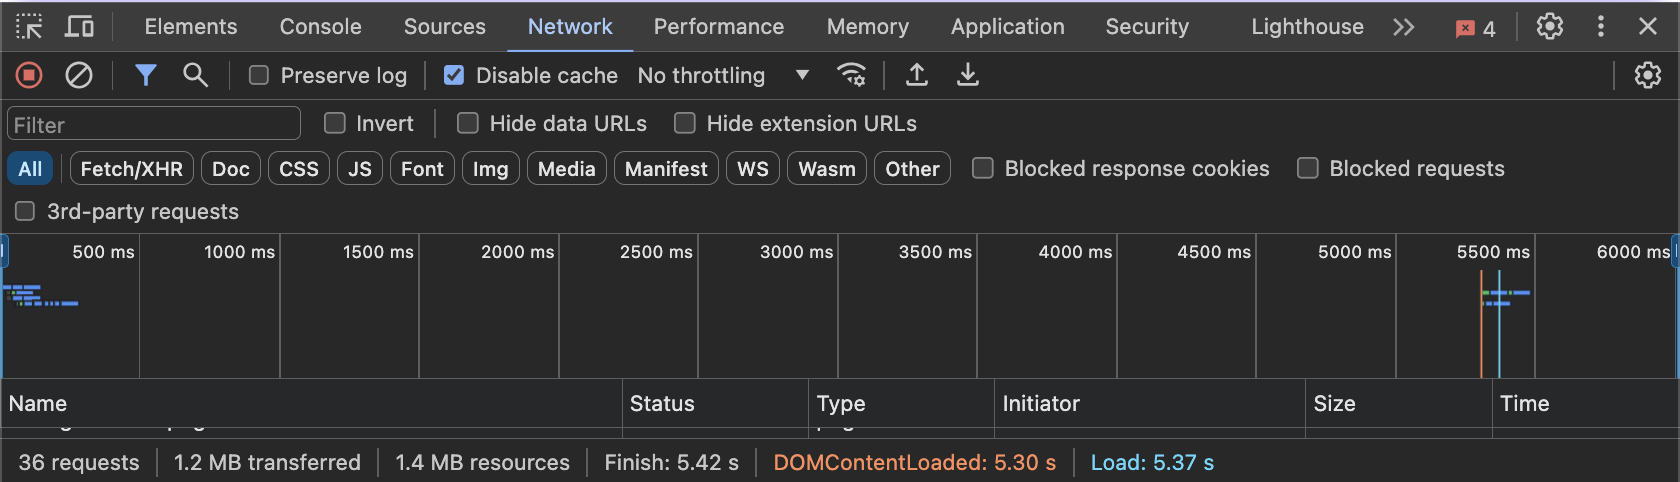
\includegraphics[width=100mm]{performance-before-user-tests.png}
    \caption{Performance Test vor Anpassungen}
    \label{img:PerformanceTestBefore}
\end{figure}

Auf der Grafik \ref{img:PerformanceTestBefore} ist zu sehen, dass der Seitenaufbau der früheren Version sehr lange dauerte.
Dies bestätigen mehrere Feedbacks der Nutzer, später mehr dazu.

\begin{figure}[!htb]
    \centering
    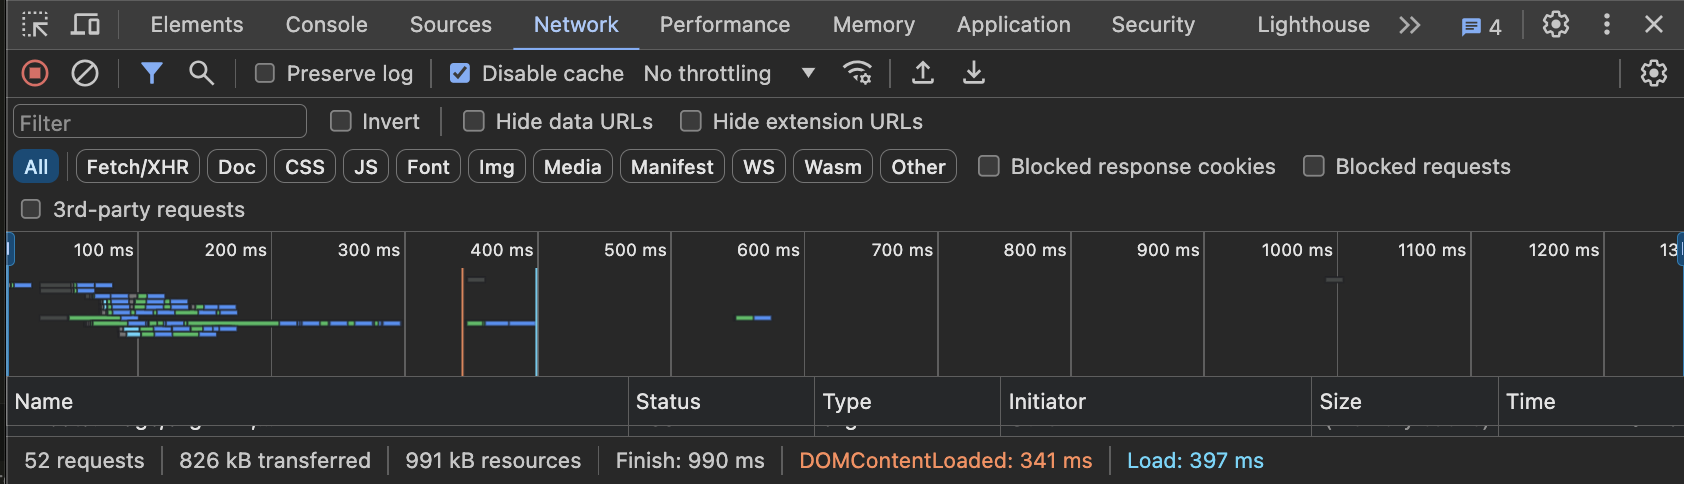
\includegraphics[width=100mm]{performance-after-user-tests.png}
    \caption{Performance Test nach Anpassungen}
    \label{img:PerformanceTestAfter}
\end{figure}

Der Vergleich zwischen Abbildung \ref{img:PerformanceTestBefore} und \ref{img:PerformanceTestAfter} zeigt, dass die Seite um einen Faktor 13 besser ist.
Die oberen Grafik zeigt die Messung der Implementation, welche sehr viele Aktionen auf dem Renderbaum ausführt.
Ein Refactoring führt zur Verschiebung dieser Arbeiten auf den Shadow-DOM.
Dadurch verkürzt sich der Ladevorgang um vier bis fünf Sekunden.
Feedbacks zu den durchgeführten User-Tests mit Programmierern als auch Endnutzern sind im nachfolgenden Kapitel aufgeführt.


\section{User Tests}


\subsection{Programmierer}



\subsection{Formular-Ausfüller}



% Keyboard navigation. Using keyboard to narrow down possible categories/values (maybe fuzzy searching), otherwise it takes me longer to find something than compared to a standard dropdown, even if the list there is bigger.
% Teams Nachricht an Lea ;)
% ich finde es etwas unintuitiv beim SelectComponent neben den offensichtlich verständlichen selectAttriutes (labl, name, numberOfColumns) noch ein Callback mitzugeben.

% ich hätti mir mehr beschreibung gewünscht wie ich die komponente verwenden muss. (ich musste eher dannach suchen.
% Bessere Dokumentation war verwirrend (Code).
% - Doku: In der Code Doku von SelectComponent dürfte der Return Value besser beschrieben werden (welches Array Element ist was). Das wird erst in den Anwendungsbeispielen klar.
% - Detail: numberOfColumns ist etwas "verbose"
% Es würde helfen, wenn die Types im JSDOC spezifiziert wären und wenn die Library eingebunden wäre. Dann wäre die Dokumentation leichter auffindbar.
% War mir am Anfang nicht klar dass was SelectComponent() zurückgibt und ob das Input-element sowie dass label-element selbst erstellt werden soll. Danach war es intuitiv anzuwenden.

% ---------

% Nitpicking: while I see why the component is imported from a URL for the user tests, it makes it hard to use on a spotty network.
% ich persönlich hatte zu beginn schwierigkeiten zu verstehen wie das "framework" funktioniert. die beschreibung für die tasks (ab task2) sind zum teil etwas unklar =>

% The value data is provided by the function `Service.getRegionsByCountry()`,
% the categories are provided by the function `Service.getCountries()`

% RegionsByCountry muss man noch das Country mitgeben. Hätte in der beschreibung drinstehen können.

% ----------

%  Isch s selectAttributes `numberOfColumns` wörklich nötig? Ih be nämlich chli am umespiele gsii, met was passiert wenn mer `numberOfColumns` uuf en "falsche" Wert setzt oder eifach meh/weniger `serviceCallbacks` mit git. Vo mir uus gseh, chönt mer `numberOfColumns` vo  `serviceCallbacks.length` ableite...?
%  Ehr hend nah recht es performance Problem wenn d liste lang isch...Dur s implementiere vo Task 2.2 brucht d websiite ca. 5 sekunde zum lade (rein Javascript execution). Das liht ned ahm Javascript, sondern am HTML rendering sowiit ih gseh ha. Ha suscht nah e Performance Trace gmacht wo mer in Chrome chan drii lade ahhghänkt.
%  Isch betz speziell, dass `serviceCallbacks` array in vercherter reihefolg muen drii geh werde wies denne ahhzeigt wird...
%  Wenn mer 2 Kollone het, aber rechts ke uuswahl, de chan mer au nüt uuswähle... Ja isch z erwarte aber isch au ih de Demo vorhande
%  För mich isch ned immer klaar gsii, wenns nah meh optione unde oder obedraa het. Ih de Browser Dropdown liste gseht mer das sehr schnell dur pfiili obe und unde


\section{Diskussion}

% herausforderungen
% komplexeste probleme
% erfolge
% unerwartete wendungen
% entscheidungen, gründe => kein filter/ suche

\section{Fazit}
